%%%%%%%%%%%%%% ENCABEZADOS %%%%%%%%%%%%%%%%
%ENCABEZADO - PARA ARTICULO
\documentclass[11pt,a4paper,spanish]{article} %NOTA - ARTICLE NO PUEDE TENER \CHAPTER
\usepackage[english]{babel}
\usepackage{babel}
\usepackage[T1]{fontenc}
\usepackage{textcomp}
\usepackage{multicol}
\usepackage{graphicx}
\usepackage{geometry}
\usepackage{makeidx}
\usepackage{appendix}
%\usepackage{showframe} 
\usepackage{setspace}
\usepackage{adjustbox}
\usepackage[nottoc]{tocbibind}
\usepackage[utf8]{inputenc} % Puede depender del sistema o editor
\usepackage{natbib}
\usepackage{amsfonts}
\usepackage{amsmath}
\usepackage{calc}




%Declaramos los parrafos
\setcounter{tocdepth}{4}
\setcounter{secnumdepth}{4}




%Estilo de la biografia
\bibliographystyle{apalike}


%MÁRGENES
\geometry{
 a4paper,
 total={170mm,257mm},
 left=30mm,
 top=25mm,
 right=30mm,
 bottom=25mm
 }
 
%ÍNDICE
\makeindex 

 
%COMIENZO DEL DOCUMENTO
\begin{document}
\nocite{*}

%PORTADA
\begin{titlepage}
    \begin{center}
        \vspace*{6cm}
        \Huge
        \textbf{Competición de Kaggle.com: \\
        Santander Costumer Satisfaction}
        \vspace{1cm}
        
        \LARGE
        por
        
        \vspace{1cm}
        \textbf{José Domingo Mateo Vázquez}
        \vfill
        \normalsize
        Tesis presentada en conformidad con los requisitos del \\
		 Máster en economía, finanzas y computación.


        \Large
        
        
        \vspace{1cm}
        
        Universidad de Huelva  
        
        Universidad Internacional de Andalucía  
        
        Noviembre de 2017
          
        \begin{figure}[b]
			\begin{multicols}{2}
   				 
\includegraphics[scale=0.3]{logouhu.eps}\par 
   				 \hfill
    			 
\includegraphics[scale=0.4]{logounia.eps}\par 
    		\end{multicols}
		\end{figure}
	
    \end{center}
\end{titlepage}


%PAGINA DEL ABSTRACT
\begin{center}
\Huge
\textbf{Competición de Kaggle.com: \\
Santander Costumer Satisfaction}
\vspace{1.25cm}

\normalsize
\textbf{José Domingo Mateo Vázquez}

Máster en economía, finanzas y computación

\vspace{0.5cm}
Supervisado por:

\textbf{José Manuel Bravo Caro}

Universidad de Huelva y Universidad Internacional de Andalucía

2017

\vspace{1cm}

\abstract{This MSc. final project brings a solution to the kaggle's Santander Customer Satisfaction problem. This is a supervised machine learning's problem about the prediction of client’s satisfaction. Some algorithms and their libraries were used to explore a solution. The programming language used was R.} 

\vspace{2cm}

\textbf{JEL Classification:}  C53, C55, C88, D12, M37

\vspace{0.5cm}

\textbf{Keywords:}  Machine Learning, Supervised Learning, Binary Classification, AUC, Imbalanced Classes, R, Logit, SVM, KNN, Naïve Bayes, XGBoost 

\vspace{2cm}

\selectlanguage{spanish} 
\abstract{Este proyecto final de máster aporta una solución al problema Santander Customer Satisfaction de la plataforma kaggle.com. Es un problema de aprendizaje automático que se encuadra dentro del aprendizaje supervisado y consiste en la predicción de la satisfacción de los clientes del Banco Santander. Se han utilizado diferentes algoritmos programados en el lenguaje de programación R así como diferentes librerías.} 

\end{center}
\newpage % Nueva página


%AGRADECIMIENTOS - DEDICATORIA
\vspace*{3cm}
\begin{flushright}
\textit{A todxs lxs que me\\
ayudaron a llegar hasta aquí.}
\end{flushright}
\newpage

%ÍNDICE
\selectlanguage{spanish} 
\doublespacing %Ponemos el interlineado doble
\tableofcontents
\newpage % Nueva página


%LISTA DE TABLAS
\renewcommand{\listtablename}{Índice de tablas}
\listoftables
\newpage

%LISTA DE GRÁFICOS
\renewcommand{\listfigurename}{Índice de gráficos}
\listoffigures
\newpage

%Ponemos el interlineado a 1.3 y añadimos espacio entre párrafos
\setlength{\parskip}{1em}
%\setstretch{1.3}

\singlespacing %Volvemos a poner el interlineado simple

%TEXTO
\section{Introducción}
El análisis de datos es uno de los campos con más proyección profesional en la actualidad. El estudio y extracción de información de grandes cantidades de datos y la elaboración de modelos capaces de predecir de forma fidedigna procesos cuya apariencia apriorística toma matices vastos y caóticos se ha convertido en una prioridad para un mundo empresarial temeroso de la incertidumbre propia de los asuntos económicos. 

Éste de repente ha visto como la evolución de las tecnologías de la información ha permitido que sea posible la generación y almacenaje de grandes volúmenes de datos a costes muy pequeños. Pero este almacenaje no ha conseguido en muchas ocasiones crear beneficios tangibles para las empresas puesto que la extracción de información útil de los datos es un proceso complejo, pesado y heterogéneo, cargado de contingencias y eventualidades que pueden hacer que con los mismos datos y pequeñas diferencias en su tratamiento y en la construcción de modelos predictivos se puedan llegar a obtener millones de modelos con resultados totalmente diferentes entre sí. 

\subsection{¿Qué problema escoger?}
La elección del problema es la elección más trascendental de todo el proyecto. La principal limitación que tenemos es la temporal. La docencia del máster finaliza a mediados de julio y el proyecto final ha de ser presentado en septiembre u octubre, por ello el tiempo efectivo para la realización del proyecto es aproximadamente dos meses y medio. En este tiempo deberemos tener listo todos los elementos del proyecto: análisis, redacción, presentación, etc. 

El máster está orientado al análisis económico, por ello hemos trabajado especialmente los métodos de análisis, algoritmos, etc. relacionados con este campo, por este motivo sería recomendable que el problema final estuviese relacionado con la economía o a la empresa. 

En tercer lugar, la dificultad del problema ha de ser lo más alta posible. En este sentido el proyecto ha de ser entendido como un reto personal, en el que exprimir al máximo las capacidades aprendidas en el máster y el conocimiento del tutor, para desarrollar la capacidad resolutiva de las diferentes problemáticas que se irán dando a medida que avancemos en la investigación.  

Por último, el problema deberá ajustarse lo máximo posible a la realidad. La idea es encontrar una base de datos real con un problema que responda a las necesidades que tienen las empresas, en el que la experiencia que ganemos en su resolución pueda ser utilizada en otros problemas y campos similares. 


\subsection{La elección final}
Por los motivos anteriormente expuestos, la elección final consistirá en la búsqueda de solución a un problema prioritario para las empresas: ¿Es posible saber con antelación la insatisfacción de los clientes?. Para ello van a utilizarse los datos del Banco Santander aportados a la competición "Santander Customer Satisfaction" de la web kaggle.com. (https://www.kaggle.com/c/santander-customer-satisfaction).

Kaggle es una web que dispone de numerosas bases de datos y en las que se realizan competiciones. El problema escogido se corresponde a una competición que ya finalizó, de esta manera evitaremos problemas con los tiempos del proyecto final y los tiempos establecidos para la competición. 
  
El objetivo general es hacer un estudio del problema planteado, identificar la naturaleza y características de sus elementos, explorar las posibles soluciones con sus ventajas e inconvenientes y por último proponer una solución que satisfaga las necesidades de la problemática planteada y ponerla en contexto con el resto de soluciones aportadas.

 

\subsection{Sobre kaggle.com}
Kaggle es una plataforma web dedicada a la ciencia de datos. En ella se realizan competiciones en las que diversos equipos proponen soluciones a problemas planteados por empresas, organismos, ... interesados en la extracción de información valiosa de sus datos. Numerosas empresas han invertido en esta plataforma, que se ha convertido en una forma de poner en contacto y organizar a los analistas de datos mas talentosos del mundo, y hacerlos accesibles a organizaciones de cualquier tamaño.
  
Estadísticos, analistas de datos e investigadores de varios campos participan en esta comunidad que sumaba en mayo de 2016 536.000 usuarios alrededor de 194 países. Los motivos para participar son varios: la cuantiosa cifra de los premios de sus competiciones, la facilidad de uso de su web, sus foros de debate donde participan desde estudiantes hasta miembros de los equipos de desarrollo de DeepMind de Google, ..., pero sobre todo esta plataforma ofrece un espacio en el que comprobar e investigar como otros analistas han afrontado la resolución de problemas complejos relacionadas con infinidad de problemáticas dentro del campo del análisis de datos.

La mecánica de una competición de kaggle es la siguiente:

1. El promotor de la competición elabora los datos y la descripción del problema. Los datos son anonimizados.

2. Los participantes trabajan con los datos, elaboran modelos y compiten entre ellos para ver quién es capaz de realizar el mejor modelo. Los trabajos se envían a la web y son puntuados mediante el cotejo con un archivo de solución final. La puntuación obtenida es usada para formar un ranking con los participantes.

3. Después de que acabe el plazo de la competición, el promotor se hace cargo del pago del premio y a cambio obtiene la explotación mundial a perpetuidad de la entrada ganadora. 

El resultado de las más de 200 competiciones que kaggle ha llevado a cabo desde su fundación ha sido diversa: investigación de proyectos sobre la investigación del SIDA, la predicción del tráfico, predicción de gustos, papers académicos, etc. 

Las competiciones no siempre tienen como premio beneficio económico, también se han realizado competiciones en las que el premio ha consistido en entrevistas de trabajo en empresas punteras en el análisis de datos.

 

\subsection{Sobre el Banco Santander}
El Banco Santander es un banco español con sede en la ciudad de Santander (Cantabria). Su presidenta es Ana Patricia Botín. Es un banco con más de 150 años de historia. En él trabajan un total de 188.492 empleados. Su clientela es muy vasta, y la forman más de 125 millones de clientes. Posee casi 4 millones de accionistas. Su capitalización bursátil es de 72.314 millones de euros y el beneficio total que obtuvo en el año 2016 ascendió a 6.204 millones de euros. El Banco Santander realiza también labores sociales. Concedió 36.684 becas de estudio y posee acuerdos con 1.183 universidades e instituciones académicas de 21 países. 

Es un banco internacionalizado que se organiza mediante un modelo de filiales autónomas que son gestionadas en función de criterios y equipos locales y que tiene actividad en todo el mundo. Sus principales focos de negocio los encontramos en Europa y América. Sus mercados principales son: España, Alemania, Polonia, Portugal, Reino Unido, Brasil, México, Chile, Argentina y Estados Unidos. Tiene también una cuota de mercado significativa en Uruguay y Puerto Rico. 

Su modelo de negocio está orientado a la satisfacción de diferentes tipos de clientes: particulares, empresas, corporaciones privadas, entidades públicas... 

El Santander es el segundo banco por capitalización de la eurozona y decimonoveno del mundo. Es la segunda marca española más valiosa y la número 70 del mundo con un valor de marca de 6.223 millones de dólares.



\subsection{Acerca de la competición Santander Customer Satisfaction}
La satisfacción de los clientes es una de las medidas clave del éxito de las empresas. Los clientes insatisfechos abandonarán la empresa en el primer momento que les sea posible. Por otra parte, es muy difícil captar su insatisfacción antes de que se produzca el abandono definitivo de la empresa, ya que rara vez la demuestran antes de abandonarla.

En esta competición de kaggle el Banco Santander buscaba modelos que fuesen capaces de identificar a los clientes insatisfechos de forma temprana, con la finalidad de implementar medidas y mecanismos proactivos que mejorasen la opinión de sus clientes antes de que cortaran sus servicios con el Banco Santander y acabasen en sus competidores. 

La evaluación de los modelos se llevará a cabo mediante el área bajo la curva ROC existente entre la probabilidad predicha y la realidad observada.

Esta competición tuvo lugar entre finales de abril y principios de mayo de 2016. Los premios ofrecidos por el Banco Santander ascendían a un total de 60.000 dólares, repartidos entre los tres primeros clasificados a razón de 30.000 dólares para el mejor modelo, 20.000 dólares para el segundo y 10.000 dólares para el tercero. 

Por último, mencionar que en total participaron 5.123 equipos diferentes. El equipo ganador fue el Shize \& Nir, formado por los usuarios Shize Su y Medrr, con una puntación de 0.829072. El segundo clasificado fue el usuario kg\_joi con una puntuación de 0.829063. Por último, el tercer equipo clasificado fué el \#1 Leustagos formado por un total de 11 usuarios con una puntuación de 0.828530.


\subsection{Sobre la Base de Datos}
La base de datos aportada para la competición por el Banco Santander tiene un total de 151.838 registros. Ésta ha sido dividida en dos grupos de datos: los datos de entrenamiento y los datos de test. Esta división es la usual dentro del campo del análisis de datos. 

Los datos de entrenamiento lo forman un conjunto de datos que son usados para establecer las relaciones existentes entre los datos y realizar (o entrenar) los modelos predictivos. 
Los datos de test en cambio son aquellos datos que son usados para evaluar la calidad de las predicciones que el modelo que hemos realizado es capaz de hacer.

La división de la base de datos original en estos dos subconjuntos de datos ha sido realizada con una proporción aproximada del 50%, lo que quiere decir que un 50% del total de los datos han sido destinados al subconjunto de entrenamiento y el otro 50% al subconjunto de test.

En lo que respecta a las variables, la base de datos tiene un total de 370 variables. Tenemos además que otra variable nos indica si el cliente estaba satisfecho o no. Esta es la variable que tendremos que predecir con el resto de variables. En este caso nos han proporcionado esta variable en los datos de entrenamiento, pero no en los de test. El motivo es que el grado de acierto que obtengamos al predecir ésta será el instrumento que kaggle utilizará para clasificar los modelos predictivos realizados en función de su calidad de predicción. 

Por otra parte, en lo que respecta a la naturaleza de las variables hay un elemento fundamental que va a condicionar muchísimo nuestro análisis, y es que vamos a trabajar a ciegas ya que las variables están numeradas y no tenemos información sobre su significado, por lo que podremos clasificar los modelos en función de su calidad de predicción, pero no podremos sacar conclusiones cualitativas sobre los motivos, indicadores o razones que llevan a la insatisfacción de los clientes. También aumenta la dificultad a la hora de crear nuevas variables cualitativas que reflejen cuestiones económicas, políticas, sociales, de actualidad, etc. que puedan tener influencia sobre la satisfacción de los clientes.

Posteriormente entraremos en profundidad en el análisis pormenorizado de las características de las variables. 

\subsection{Objetivos}
El objetivo principal de este trabajo es aprender lo máximo posible y demostrar la capacidad de trabajar, plantear y resolver este tipo de problemas. La idea es la de aprender cómo funcionan los algoritmos y ser capaz de construirlos. 

Otro objetivo personal es el aprender el lenguaje de programación R. Hasta ahora había venido trabajando con python y matlab. R es uno de los lenguajes más usados dentro del mundo del análisis de datos. Tener un buen nivel en éste y conocer su idiosincrasia es fundamental. 

En lo que respecta a la competición, el objetivo es aportar un modelo con la puntuación más alta posible, la idea es obtener un modelo que obtenga una puntuación que al menos sea similar a la obtenida por el ganador de la competición. Una puntuación mucho más baja demostraría la falta de capacidad personal y por lo tanto supondría un fracaso. 


\section{Modelos predictivos: Algoritmos y evaluación}

En este apartado se expondrán brevemente una serie de conceptos: el campo en el que se encuadra el trabajo, los algoritmos utilizados, las métricas de evaluación de los resultados, etc.


\subsection{Técnicas de aprendizaje automático: Aprendizaje supervisado}
El aprendizaje automático o machine learning se encuadra dentro de la inteligencia artificial y es la rama de las ciencias de la computación que se encarga de crear programas capaces de aprender y tomar decisiones por sí mismos. 

El aprendizaje de estos programas es posible gracias a que son capaces de detectar patrones dentro de los datos y mediante la aplicación de modelos estadísticos y otros algoritmos es posible predecir o estimar características. 

Los modelos de aprendizaje automático suelen enfocarse en la predicción, por ello es más difícil interpretar sus resultados que con los modelos estadísticos. Estos suelen tener coeficientes que sirven para explicar las causas y el nivel de influencia de las variables.

Hay diferentes tipos de algoritmos de aprendizaje automático: los de aprendizaje supervisado, los de aprendizaje no supervisado... Por las características de nuestro problema vamos a hacer uso de los algoritmos de aprendizaje supervisado. 

Los algoritmos de aprendizaje supervisado son utilizados para clasificar nuevos datos. Se caracterizan porque el algoritmo para aprender necesita datos que hayan sido previamente clasificados.  El algoritmo analiza los datos de entrenamiento e infiere una función que puede ser utilizada para clasificar nuevos datos. Algunos de los algoritmos de aprendizaje supervisado que podemos encontrar son los siguientes: 

\begin{itemize}

	\item{Máquinas de soporte vectorial (SVM)}
	\item{Regresión logística}
	\item{Redes Neuronales}
	\item{Vecinos más cercanos (KNN)}
	\item{Métodos basados en árboles de decisión:}
	
		\begin{itemize}
			\item{Random Forest}
			\item{C4.5}
			\item{GBM}
			\item{XGBoost}
			\item{Etcétera}
		\end{itemize}
		
	\item{Clasificador Bayesiano Ingenuo (Naïve Bayes)}
	\item{Etcétera}

\end{itemize}

En este trabajo vamos a hacer uso de la regresión logística, clasificador bayesiano ingenuo, máquina de soporte vectorial, vecinos más cercanos, Random Forest y XGBoost. A continuación se describirán brevemente las características de cada uno de estos algoritmos. 

\subsubsection{Regresión Logística}
Cómo en nuestro caso la variable dependiente es una variable binaria podemos modelizarla mediante el uso de un modelo de regresión logística. Este modelo fue desarrollado por David Cox y se usa para medir la relación entre una variable dependiente categórica y una o más variables independientes por medio de la estimación de probabilidades utilizando una función logística, es decir, nos ayuda a medir como influyen las variables independientes a la hora de determinar la probabilidad de que ocurra un suceso determinado y utilizar esto para realizar predicciones. 

La probabilidad aproximada del suceso se aproximará mediante una función logística que puede reducirse al cálculo de una regresión lineal para la función logit de la probabilidad. La función logit se utiliza para mantener la salida de la función entre 0 y 1:

$$P(z) = \frac{1}{1 + \exp(-z)}$$

Asumimos que $z$ es una función lineal con una única variable independiente $x$. Podemos expresar $z$ de la siguiente forma:

$$z = \beta_0 + \beta_1 x $$

$z$ también puede expresarse como una combinación lineal de diferentes variables explicativas:

$$z = \beta_0 + \beta_1 x_1 +  ... \beta_n x_n $$

La función logística puede entonces ser escrita así:

$$F(x) = \frac{1}{1+ \exp-(\beta_0 + \beta_1 x_1,i + ... \beta_n x_n,i)}$$

Pues bien, la regresión logística se distingue en de la regresión lineal y de otros tipos de análisis de regresión usados para salidas binarias es la forma en la que se lnlaza la probabilidad de una salida particular con la función de prediccion lineal:

$$\mbox{logit}(\mathbb{E}[Y_i | X_i]) = \mbox{logit}(p_i) = \ln{\left(\frac{p_i}{1-p_i}\right)} = \beta · X_i $$ 

Una de las limitaciones de este modelo es que se usa para determinar la probabilidad de pertenencia de un sujeto a una categoría determinada, por lo que no es un modelo adecuado en el caso de que la variable dependiente sea continua. En nuestro caso trabajaremos con la regresión logística binomial. Este modelo se caracteriza porque su salida puede tomar valores entre 0 y 1. En nuestro caso el 0 representa la satisfacción del cliente con nuestra empresa mientras que el 1 representará su insatisfacción.

\newpage

La regresión logística puede tener una o más variables independientes. Éstas pueden ser variables continuas o variables categóricas. 


\subsubsection{Vecinos más cercanos}
El clasificador $k$-NN es un algoritmo que se encuadra dentro de los métodos de clasificación supervisada. Funciona tanto para predecir variables categóricas como continuas y sirve para predecir los valores de una variable en función del valor de sus vecinos, es decir, de los valores que tienen las observaciones más próximas. 

Este algoritmo asume que todas las observaciones son puntos en un espacio de dimensión n, entonces, será el vecino más cercano aquel que se encuentre más próximo según la distancia Euclidiana estándar, es decir, la distancia entre dos puntos en un plano cartesiano.

$$d(X,Y) = \sqrt{\sum_{i=1}^n(x_i - y_i)^2}$$

Habremos de elegir también el valor de la variable $k$,  el número de vecinos que tendrán influencia a la hora de determinar la clase de nuestras predicciones. La elección del valor de $k$ dependerá del tipo de datos que tengamos. Valores grandes de $k$ reducen el ruido en la clasificación, pero podemos caer en el sobreajuste de los datos, es decir, que las predicciones sean buenas para el conjunto de entrenamiento pero no para datos exógenos a esta. El $k$-NN estima el valor de las predicción a través de una función de densidad de probabilidad.

Es un algoritmo que para funcionar requiere cumplir una serie de pasos:

\begin{enumerate}
	\item{Si nuestra variable dependiente es categórica, habrá que convertir las categorías a números.}
	
	\item{Las variables han de estar estandarizadas, ya que el algoritmo es muy sensible a la diferencia de escalas y tiene a sobrerrepresentar las observaciones con valores altos.}
	
	\item{Una vez que hemos calculado la matriz de distancias tendremos que escoger el número de vecinos.}
	
	\item{Por último, la observación es clasificada en función del valor de sus vecinos.}
\end{enumerate}



\subsubsection{Clasificador Bayesiano Ingenuo}
El clasificador bayesiano ingenuo o naïve Bayes, es un clasificador que se basa en el teorema de Bayes. Este modelo es denominado ingenuo porque asume la hipótesis de que las variables usadas para predecir son independientes entre sí.

El teorema de Bayes proporciona una forma de calcular la probabilidad a posteriori $P(c|x)$ con $P(c)$, $P(x)$ y $P(x|c)$. El clasificador bayesiano ingenuo asume que el efecto del valor de un predictor $x$ para una clase dada $c$ es independiente de los valores de los otros predictores. Es lo que llamamos independencia condicional de clase. La fórmula de este algoritmo es la siguiente:

$$P(c|x) = \frac{P(x|c) P(c)}{P(x)}$$

Es un método que sirve para calcular la probabilidad de que un objeto a clasificar pertenezca a una clase determinada.

Este clasificador no requiere la estimación de ningún parámetro y a veces mejora los resultados que se obtienen con métodos más sofisticados, especialmente en dos casos: cuando los atributos son totalmente independientes o cuando los atributos son totalmente dependientes. En la práctica esto se da cuando existe una separación grande entre las medias de las variables. Sería en los casos intermedios entre estos dos supuestos cuando los resultados aportados por este algoritmo no serían buenos.   



\subsubsection{Máquina de soporte vectorial}
Las máquinas de soporte vectorial son algoritmos de aprendizaje supervisado que se usan en problemas de clasificación y regresión. 

Las máquinas de soporte vectorial son sistemas que usan el espacio de hipótesis de una función lineal en un espacio hiperdimensional, entrenados con un algoritmo de la teoría de optimización que implementa un sesgo de aprendizaje derivado de la teoría estadística.

La máquina de soporte vectorial utiliza un conjunto de datos de entrenamiento para construir un modelo que separe las clases de los datos a clasificar en dos espacios lo más grande posibles mediante el uso de uno o varios hiperplanos de separación. La solución del hiperplano es la combinación de unos puntos de entrada llamados vectores de soporte. Entonces, lo que hace el algoritmo es buscar el hiperplano que mejor separa los datos, es decir, la búsqueda del mejor clasificador equivale a un problema de optimización en el que hay que maximizar el margen entre las clases. La formulación del problema sería la siguiente:
\begin{align*}
\min _{\gamma, w, b}&\quad \frac{1}{2} ||w||^2 \\
		& \mbox{s.a} \quad y^{(i)}(w^T x^{(i)} + b) \ge 1, \ i=1, ..., m
\end{align*}

Una vez se tienen nuevas muestras, se pueden clasificar en función del lugar que ocupen con relación a los hiperplanos de separación. 

El SVM es un algoritmo que funciona bien cuando existe un margen claro de separación entre las categorías y es eficiente en espacios de alta dimensionalidad pero ineficiente con bases de datos grandes, porque su tiempo de entrenamiento es bastante alto.\footnote{Se puede consultar un análisis más profundo sobre este algoritmo en https://goo.gl/KPTCML}

\subsubsection{Métodos basados en árboles de decisión}

Los árboles de decisión son un modelo predictivo que clasifica el valor de una variable de destino en función de un conjunto de variables de entrada.  

Los árboles de clasificación están compuestos por las hojas, que representan las clases a la que pertenecen las observaciones y ramas, que representan el conjunto de características mediante los cuales se deducen esas etiquetas.

Los árboles de decisión pueden ser fácilmente representados de forma visual. Por otra parte son fácilmente paralelizables, por lo que son fácilmente escalables y por lo tanto son algoritmos que suelen usarse en entornos de big data. 

El principal problema de los árboles es que  suelen tener valores altos de varianza o sesgo. 

\paragraph{Random Forest}  .


El random forest es un algoritmo predictor que utiliza la técnica de agregación de bootstrap o bagging para entrenar árboles. En el algoritmo de bagging para los árboles dado un conjunto de entrenamiento $X = x_1, ..., x_n$ con un conjunto de respuestas $Y = y_1, ..., y_n$, haciendo bagging repetidamente un número B de veces selecciona una muestra aleatoria de reemplazamiento del conjunto de datos de entrenamiento y ajusta árboles a estas muestras.

Para $b = 1, ... B$ se utilizan muestras con reemplazamiento un número $n$ de muestras extraídas de $X$ e $Y$ llamadas $X_b$ e $Y_b$. Posteriormente se entrena un árbol de clasificación o regresión $f_b$ para $X_b$ e $Y_b$. 

Después del entrenamiento, las predicciones para los datos de test $x'$ pueden realizarse utilizando la media de las predicciones de todos los árboles de regresión para x':

$$\hat{f} = \frac{1}{B} \sum_{b=1}^B f_b(x')$$

En el caso de un problema de clasificación, se toma la clase predicha que resulte mayoritaria. Este procedimiento mejora el desempeño del modelo porque disminuye la varianza del modelo sin incrementar el bias.

El número de árboles entrenados es un parámetro libre. 

El random forest se parece mucho al bagging, pero difiere en que en el proceso de aprendizaje selecciona un subconjunto aleatorio de las características del dataset. El efecto que tiene es que si existen características con una alta capacidad predictiva de la variable dependiente, éstas seran seleccionadas en muchos de los conjuntos de árboles $B$ entrenados. Generalmente, dado un conjunto de datos con un número $p$ de características, para los problemas de clasificación suele usarse un número $\sqrt{p}$ de características en cada división, mientras que para los problemas de regresión suele usarse $\frac{p}{3}$.

Random Forest es un algoritmo bastante bueno para hacer predicciones, ya que generaliza bastante bien y no suele sobreajustar los datos de entrenamiento. Además, es eficiente con grandes volúmenes de datos, problemas no balanceados, problemas con muchas variables, etc. 

Suele usarse también para estimar la importancia de las variables. 

\paragraph{XGBoost}  .

Los algoritmos de árboles basados en el boosting utilizan la media ponderada de varios árboles para intentar combinar sus resultados. En este caso los árboles se van levantando de forma lineal, uno tras otro, con la idea de que los nuevos árboles vayan mejorando los aspectos que el resto de árboles no han sido capaces de clasificar.

XGBoost es una librería que utiliza este tipo de árboles. Actualmente es una de las librerías más usadas para realizar clasificaciones. Su uso se ha extendido muchísimo y es usado por numerosas compañías. Las razones por las que su uso se ha extendido son varias:

\begin{itemize}
	\item{Soporta regresión, clasificación, etc.}
	
	\item{Está implementado en múltiples lenguajes como C++, Python, R, Java, Scala...}
	
	\item{Permite la computación distribuida.}
	
	\item{Funciona en Windows, Linux, OS X y plataformas en la nube.}

	\item{Ha resultado ser el algoritmo usado en muchas competiciones de machine learning.}
	
	\item{Está muy bien optimizado y su rendimiento es bastante bueno.}
	
\end{itemize}

Dado un conjunto de datos $x_i$ para predecir una variable objetivo $y_i$, se necesita definir una función objetivo que sea capaz de medir el desempeño de un modelo con un determinado conjunto de parámetros. Las funciones objetivo siempre contendrán dos partes: la función de pérdida y la regularización.

$$\mbox{Obj}(\Theta) = L(\theta)+\Omega(\Theta)$$

Dónde $L$ es la función de pérdida para el entrenamiento y $\Omega$ el término de regularización. La función de pérdida mide cómo predice nuestro modelo los datos de entrenamiento. Un ejemplo de función de pérdida sería el error cuadrático medio. El término de regularización controla la complejidad del modelo y ayuda a reducir el sobreajuste. El principio general que debe guiarnos es querer un modelo simple y predictivo. 

XGBoost utiliza un modelo de conjunto de árboles de clasificación y regresión (CART). Frente a los árboles de decisión dónde las hojas únicamente contienen valores de decisión, en los modelos CART una puntuación está asociada a cada una de las hojas. Las puntuaciones de predicción de cada árbol individual se suman para obtener la puntuación final. De esta manera los árboles se complementan entre ellos. Matemáticamente el modelo puede expresarse así:

$$\hat{y}_i = \sum_{k=1}^K f_k(x_i), f_k \in \nabla$$

$K$ es el número de árboles, $f$ es la función en el espacio funcional $F$, y $F$ es el conjunto de todos los posibles CARTS. Entonces nuestro objetivo a optimizar puede ser escrito como:

$$\mbox{obj} (\theta) = \sum_{i}^n l(y_i,\hat{y}_i) + \sum_{k=1}^K \Omega(f_k)$$

Para entrenar el modelo se utiliza una estrategia aditiva, fijando aquello que hemos aprendido y añadiendo un nuevo árbol cada vez. Escribimos el valor de predicción en cada paso t como $\hat{y}_i^{(t)}$, así tenemos:

\begin{align*}
\hat{y}_i^{(0)}& = 0 \\
\hat{y}_i^{(1)}& = f_1(x_i) = \hat{y}_i^{(0)} + f_1(x_i)\\
\hat{y}_i^{(2)}& = f_1(x_i) + f_2(x_i)= \hat{y}_i^{(1)} + f_2(x_i) \\
&\mathrel{\makebox[\widthof{=}]{\vdots}} \\
\hat{y}_i^{(t)}& = \sum_{k=1}^t  f_k(x_i) = \hat{y}_i^{(t-1)} + f_t(x_i) \\
\end{align*}

En cada uno de los pasos se irá añadiendo el árbol que mejor optimice nuestro objetivo. 

$$\mbox{obj}^{t} = \sum_{i=1}^n l(y_i, \hat{y}_i^{(t)}) + \sum_{i=1}^t \Omega (f_i) = \sum_{i=1}^n l(f_t) + \mbox{constante}$$

En lo que respecta a la regularización tenemos que definir la complejidad del árbol $\Omega(f)$. En XGBoost la complejidad se define como:

$$\Omega(f) = \gamma T + \frac{1}{2} \lambda \sum_{j=1}^T w^2_j$$

Con todo esto, podemos escribir el valor objetivo con el árbol t-énésimo como:

$$\mbox{Obj}^{(t)} \approx \sum_{i=1}^n[g_i w_{q(x_i)} + \frac{1}{2} h_i w^2_{q(x_i}] + \gamma T + \frac{1}{2}\lambda \sum_{j=1}^T w_j^2 = \sum_{j=1}^T[(\sum_{i \in I_j}g_i)w_j + \frac{1}{2}(\sum_{i \in I_j} h_i + \lambda) w_j^2] + \gamma T$$

Por último la estructura de los árboles se determina mediante la fórmula:

$$\mbox{Ganancia} = \frac{1}{2} \left[\frac{G^2_L}{H_L + \lambda} + \frac{G^2_R}{H_R + \lambda}+ \frac{(G_L+G_R)^2}{H_L + H_R + \lambda}\right] - \gamma $$

Con esta formula comprobamos si es positiva la división de una hoja en dos nuevas hojas. Esta fórmula tiene cuatro partes: La primera parte de la fórmula es la puntuación en la nueva hoja izquierda, la segunda parte es la puntuación en la nueva hoja derecha, la tercera parte es la puntuación en la hoja original y $\gamma$ es la regularización en la hoja adicional. Podemos comprobar que si la ganancia es más pequeña que $\gamma$ no doberíamos añadir una nueva rama.

\subsection{La evaluación de los modelos: El área bajo la curva ROC (AUC)}

Existen numerosas posibilidades a la hora de evaluar la puntuación de los modelos predictivos de clasificación: porcentaje de aciertos, precisión, coeficiente de Gini normalizado... En nuestro caso vamos a utilizar el área bajo la curva ROC, también denominada AUC (Area under the curve). 

La curva ROC (Receiver Operating Characteristic), es una metodología desarrollada para analizar un sistema de decisión. Consiste en una representación gráfica, en la que contrastamos la sensibilidad con la especificidad para un sistema de clasificación binario. 

La sensibilidad es el cociente entre el número de casos verdaderamente positivos y el número de casos clasificados como positivos. 

Por su parte la especificidad es el cociente entre el número de casos verdaderamente negativos y el número de casos clasificados como negativos.

En la curva ROC se sitúa en el eje de las abscisas el valor de uno menos la especificidad y en el eje de las ordenadas el valor de la sensibilidad. Por esto, la situación ideal es estar cerca del vértice superior izquierdo, ya que en este caso habría mucha sensibilidad y especificidad.

La curva ROC nos muestra el desempeño del clasificador en todo su rango operativo. Puede ser usada para visualizar y seleccionar el mejor clasificador, aquel que por un lado maximice los verdaderos positivos y negativos y por el otro minimice los falsos positivos. En función del tipo de problema puede cambiar el criterio usado para el clasificador. 

El área bajo la curva ROC representa la probabilidad de que un clasificador ordene una instancia positiva elegida aleatoriamente más alta que una negativa. El AUC nos permite comparar clasificadores.

\newpage

\section{Abordando el problema}

Estamos ante un problema de clasificación complejo con gran cantidad de variables que habrá que resolver mediante el uso de las técnicas de aprendizaje supervisado. Hay numerosos algoritmos que podemos utilizar para la creación de modelos de clasificación: modelos de regresión logística, clasificadores bayesianos ingenuos, modelos basados en árboles, clasificadores en función de los vecinos más cercanos, clasificadores basados en el gradiente, etc. Tendremos que investigar cuáles de estos algoritmos responden mejor a nuestras necesidades.  

Podemos también intentar reducir la dimensión de nuestra base de datos mediante el uso de algoritmos de reducción de la dimensionalidad como el análisis de componentes principales. Con esto ganaríamos capacidad de procesamiento y quizás capacidad de visualización, ya que mediante este tipo de técnicas transformamos nuestro problema en un problema equivalente con menor número de variables. 

Para encontrar posibles relaciones entre las diferentes variables podemos intentar usar las reglas de asociación. Estos algoritmos sirven para encontrar correlaciones entre las variables y nos pueden ayudar a obtener conclusiones e intuiciones sobre nuestra base de datos. 

\subsection{Origen de los datos}

El Banco Santander nos proporciona a través de kaggle un conjunto de datos. Los archivos proporcionados son tres: 

\begin{itemize}

\item{\textbf{train.csv} - Es el conjunto de datos destinado al entrenamiento de los modelos. Aquí se nos proporciona la variable objetivo.}

\item{\textbf{test.csv} - El conjunto de datos sobre los que hay que realizar las predicciones con los modelos que entrenemos. Se nos evaluará en función de la precisión que obtengamos a la hora de clasificar estos datos.}

\item{\textbf{sample\textunderscore submissions.csv} - Un archivo que contiene una predicción de prueba para examinar el formato correcto en el que deberemos subir nuestras predicciones a la web.}

\end{itemize} 

Los datos están anonimizados. 

\subsection{Análisis exploratorio y enriquecimiento de los datos}
El análisis exploratorio nos permite tener una primera idea sobre las características de los datos con los que estamos trabajando. Al trabajar con 371 variables a ciegas el análisis exploratorio irá encaminado a intentar inducir el significado de estas variables y a obtener información sobre su distribución, tipo, estadísticos, etc.

  

\begin{figure}[h!]
	\begin{center}
	\includegraphics[width=3.5in]{Z_01_01_Dist_casos.pdf}
    \caption{Distribución de las observaciones en función de su clase}
    \end{center}
\end{figure}

En primer lugar, vamos a ver la distribución de casos a clasificar. La variable que nos dice la clase a la que pertenece cada observación es TARGET. Ésta es una variable de tipo binomial que toma como valores 0 y 1. El valor 0 significa que el cliente está satisfecho con el servicio del banco, mientras que el valor 1 significa que el cliente está insatisfecho. Esta es la variable que tenemos que predecir con nuestros modelos y que únicamente tenemos en los datos de entrenamiento. Podemos ver la distribución de los casos en la figura 1.

\vspace{0.5cm}

Podemos comprobar como las clases están muy descompensadas entre sí. De un subconjunto de 76.020 observaciones tenemos que hay un total de 73.012 clientes que están satisfechos con el banco, mientras que 3.008 clientes están descontentos, lo que significa que en nuestro subconjunto por cada cliente descontento tenemos unos 24 clientes satisfechos. 

\vspace{0.5cm}

Esta descompensación es un gran problema ya que altera la capacidad predictiva de algunos algoritmos. Por ello cuando vayamos a proponer soluciones y vías de actuación tendremos que tenerla en cuenta para evitar que contamine los resultados.

\vspace{0.5cm}

Pese no saber con total rotundidad su significado, las 370 variables que tenemos presentan diferentes características. Podemos ver cómo están identificadas mediante un código de variable que se estructura con las letras var y un número de dos cifras. Este código distribuye las variables en 46 grupos de variables diferentes. Se sobreentiende que éstas representan las propiedades inherentes a productos diferentes. Por ejemplo, hay 5 variables que comparten la etiqueta var1, por lo que se intuye que cada una muestra una característica específica del producto var1. 

\vspace{0.5cm}

Los grupos de variables no están compuestos el mismo número de variables. Podemos comprobar el número de variables que compone cada grupo de variables en el cuadro número 1 y podemos ver como se distribuyen las variables en cada uno de los grupos en la figura número 2.

\newpage

\begin{figure}[h!]
	\begin{center}
	\includegraphics[width=6.3in, height=\textheight,keepaspectratio]{Z_01_02_Numero_variable.pdf}
	\caption{Variables que componen cada uno de los grupos de variables.}
    \end{center}
\end{figure}

\newpage

\vspace{2cm}

\begin{table}[htbp]
\begin{center}
\begin{tabular}{|l|c|||l|c|}             \hline
  \textbf{Grupo} & \textbf{Nº de vars.}  & \textbf{Grupo} & \textbf{Nº de vars.} \\  \hline
  var1  &   5  &  var25 &   6  \\ \hline 
  var2  &   5  &  var26 &   6  \\ \hline 
  var3  &   1  &  var27 &   5  \\ \hline 
  var4  &   1  &  var28 &   5  \\ \hline 
  var5  &  10  &  var29 &  10  \\ \hline 
  var6  &   5  &  var30 &   5  \\ \hline
  var7  &   6  &  var31 &   5  \\ \hline
  var8  &  10  &  var32 &   6  \\ \hline
  var9  &   2  &  var33 &  34  \\ \hline
  var10 &   2  &  var34 &   8  \\ \hline
  var11 &   1  &  var35 &   1  \\ \hline
  var12 &  10  &  var36 &   1  \\ \hline
  var13 &  47  &  var37 &   8  \\ \hline
  var14 &   5  &  var38 &   1  \\ \hline
  var15 &   1  &  var39 &  18  \\ \hline
  var16 &   4  &  var40 &  18  \\ \hline
  var17 &  34  &  var41 &  18  \\ \hline
  var18 &   8  &  var42 &   3  \\ \hline
  var19 &   1  &  var43 &   5  \\ \hline
  var20 &   5  &  var44 &  22  \\ \hline
  var21 &   1  &  var45 &   5  \\ \hline
  var22 &   5  &  var46 &   5  \\ \hline
  var24 &   5  &        &      \\ \hline

\end{tabular}
\caption{Número de variables en cada grupo de variables}
\end{center}
\end{table}


\begin{figure}[h!]
	\begin{center}
	\includegraphics[width=\textwidth, height=\textheight,keepaspectratio]{Z_01_11_Treeplot.pdf}
	\caption{Grupos de variables. Representación gráfica de su peso sobre el total de variables.}
    \end{center}
\end{figure}

\newpage

Además de este código, nuestras variables poseen una serie de etiquetas. Todos los grupos de variables poseen estas etiquetas salvo 5 de ellos. Estas etiquetas determinan la tipología de las variables. Podemos comprobar la relación de variables con sus tipos y sus etiquetas en el cuadro número 2.

\vspace{1.5cm}

\begin{table}[htbp]
\begin{center}
\begin{tabular}{|l|c|c|c|c|} \hline 
\textbf{Tipo de variable} & \textbf{Categóricas}  & \textbf{Continuas} & \textbf{Discretas} \\  \hline
Total de variables  & 3           &  123    & 244   \\  \hline
                    &             &  imp    & imp   \\  
 Prefijos asociados & Sin prefijo &  saldo  & ind   \\
                    &             &  delta  & num   \\
                    &             &         & delta \\  \hline
\end{tabular}
\caption{Tipo de variables}
\end{center}
\end{table}


Por otra parte, al no ser constante el número de variables que componen los grupos de variables, tenemos que cada uno de ellos posee una naturaleza diferente, la figura número 3 muestra la composición de cada uno de los grupos de variables, así como el número de variables de cada tipo que lo componen. 

\vspace{0.8cm}


\begin{figure}[h!]
	\begin{center}
	\includegraphics[width=\textwidth]{Z_01_03_Grafico_etiquetas_variables.pdf}
    \caption{Composición y número de variables que componen los grupos de variables.}
    \end{center}
\end{figure}


\newpage

Además, las etiquetas tienen a su vez diferentes subetiquetas. En el mapa conceptual de la figura 4 aparecen representadas como se van dividiendo las etiquetas y subetiquetas de las variables.



\begin{figure}[h!]
	\begin{center}
	\includegraphics[width=\textwidth]{Z_01_04_Variables.pdf}
    \caption{Relación de etiquetas y subetiquetas de las variables}
    \end{center}
\end{figure}

\newpage


En la figura número 5 podemos ver el tipo de variable que compone cada uno de los grupos de variables, así como el número de variables de cada tipo en cada uno de ellos.  

\begin{figure}[h!]
	\begin{center}
	\includegraphics[width=\textwidth]{Z_01_05_Grafico_tipo_variables.pdf}
    \caption{Tipo y número de variables que componen los grupos de variables.}
    \end{center}
\end{figure}


En otro orden de cosas, si atendemos al contenido de cada una de las variables podemos extraer información interesante:

\begin{itemize}
  \item{Hay 3 variables que parecen que crean categorías de los datos.}
  
  \begin{itemize}
      \item{\textbf{var15} - Algunos analistas de datos \footnote{https://www.kaggle.com/c/santander-customer-satisfaction/discussion/19291} apuntan a que esta variable podría ser la edad del titular. Como argumentos a favor de esta tesis tenemos que el rango de esta variable se mueve entre 5 y 105 con valores enteros. Por otra parte, tenemos un pico de esta variable en los valores próximos a 20-25, la hipótesis es que este pico se correspondería con alumnos universitarios, ya que el Banco Santander tiene convenios firmados con distintas universidades que hace que muchos alumnos acaben abriendo su cuenta en este banco. En contra de esta tesis hay analistas que apuntan a que la variable \textbf{var38} mostraría el volumen de la hipoteca de clientes \footnote{https://www.kaggle.com/c/santander-customer-satisfaction/discussion/19895}, si hacemos una tabla de contingencia comparando estas dos variables, sucedería que todos los clientes -incluidos aquellos menores de 25 años- tendrían una hipoteca. Esto es absurdo, por lo que estas dos tesis son incompatibles entre sí.}
      
      \item {\textbf{var3} - Aparenta ser la nacionalidad del cliente. Hay 116 valores que tienen aparejada una categoría nula que habrá que modificar más adelante.}
    \end{itemize}
  
    \item{Hay un total de 75 variables binarias. Estas parecen corresponderse con productos del banco e indicarían el número de clientes que tienen contratados esos productos, o la existencia de características.}

  \item{Las variables continuas ascienden a 123. El tipo de variable contenida aquí parece indicarnos que podemos encontrar información sobre el nivel de efectivo de los clientes, el dinero que tienen en diferentes productos, nivel de intereses, algunas variaciones en el efectivo en diferentes períodos, descubiertos, etc. }
  
    \item{Las variables enteras ascienden a 169. Una gran cantidad de estas variables se mueven en múltiplos de tres. Podrían indicar trimestres.}
    
    \item{Otra información interesante:}

  \begin{itemize}
      \item{Hay un total de 34 variables con todos sus valores iguales a 0.}
      
      \item{La mayoría de las variables tienen una gran proporción de valores iguales a 0. También hay bastantes variables que de entre todos sus valores únicamente una minúscula proporción de ellos no son 0.}
      
      \item{Algunas variables que tienen el prefijo delta y otras como las variables var13, var36, etc. tienen valores que parecen ser valores nulos o perdidos.}
      
    \end{itemize}
    
\end{itemize}

\begin{figure}[h!]
	\begin{center}
	\includegraphics[width=\textwidth]{Z_01_06_Grafico_ceros_variables.pdf}
    \caption{Porcentaje y número total de variables con ceros en los grupos de variables.}
    \end{center}
\end{figure}


Tras esta evaluación se realizarán una serie de actuaciones:

En primer lugar, las variables que tienen todos sus valores iguales a 0 son prescindibles puesto que no arrojan ningún tipo de información que ayude a discriminar entre las dos clases. En todo caso, hay una información que si podría llegar a ser útil y es el número total de ceros que posee cada observación, por lo que se generará una nueva variable cualitativa que recoja el número total de ceros. Podemos ver la distribución de esta nueva variable en el histograma de la figura 7.


\begin{figure}[h!]
	\begin{center}
	\includegraphics[width=\textwidth]{Z_01_07_Historial_N_ceros.pdf}
    \caption{Histograma de la variable con el número total de ceros de cada observación.}
    \end{center}
\end{figure}


Se comprobará además la similitud de las variables restantes entre ellas, de tal manera qué si se detectan variables con valores iguales entre sí, se procederá a la eliminación de éstas hasta dejar sólo una, puesto que se entiende que la información que aportan es la misma. En total se eliminan 62 variables, quedándonos con un total de 309. En la figura 8 podemos ver las variables eliminadas y a que grupo de variables pertenecen. 

\begin{figure}[h!]
	\begin{center}
	\includegraphics[width=\textwidth]{Z_01_08_Grafico_variables_eliminadas.pdf}
    \caption{Variables eliminadas.}
    \end{center}
\end{figure}

En segundo lugar, habrá que proceder a tratar los datos perdidos o erróneos. Tras estudiar la base datos, la primera conclusión es que los datos en general están bien tratados y existen muy pocos valores perdidos o erróneos. En general tenemos que estos datos vienen representados con los códigos 99, -999999 o 9999999999. En estos casos y tras las transformaciones realizadas en la actuación anterior, hay pocas variables que contengan observaciones con estas características y estas se caracterizan por ser de tipo categórico, entero, o continuo con pocos valores. 

Para tratar los datos perdidos o erróneos pueden utilizarse varios métodos: eliminación, la sustitución por el valor de la media, la sustitución por el valor de la mediana, predecir mediante el uso del resto de variables y observaciones el valor que habría de tener el valor perdido, etc. 

En este caso, para las variables categóricas optaré por transformar los valores perdidos por el número entero siguiente a el valor más alto de cada una de las variables. El motivo por el que opté por este método es que al tratarse de categorías, puede ser que los datos perdidos no guarden ningún tipo de característica que los haga circunscribirse a las categorías existentes. De esta manera se mantiene cierto elemento diferenciador con los valores que disponemos. 

En el caso de var3, como es una variable categórica, el criterio de transformación será el de transformar los valores perdidos al primer valor de categoría libre existente. \footnote{Para los modelos basados en árboles se ha usado un conjunto de datos sin estas transformaciones ya que bajaban ligeramente la puntuación de la predicción.}

En tercer lugar, se ha procedido a normalizar y estandarizar los datos. Las variables continuas han sido transformadas, ya que tenían un rango muy alto. Se han calculado sus logaritmos \footnote{Ídem}.

En cuarto lugar, para subsanar la descompensación de observaciones en la clase objetivo existen diferentes métodos. Los más simples son los que se conocen como downsampling y upsampling. El downsampling consiste en reducir las observaciones de la clase mayoritaria, para así hacer coincidir el número de observaciones existente en cada una de las clases. Presenta el problema de que al eliminar observaciones estamos perdiendo información. 
Por otra parte, tenemos el upsampling, que viene a ser el proceso inverso del anterior, es decir, duplicar observaciones de la clase minoritaria hasta que su número coincida con aquellas de la clase mayoritaria. 

En principio este segundo método es mejor que el primero, pero además de estos existen otros métodos más avanzados: ROS, RUS, SMOTE, ROSE, etc. Estos métodos en vez de duplicar directamente las observaciones "crean" nuevas observaciones artificiales introduciendo ligeras modificaciones, pero intentando a su vez que éstas sean fidedignas a la realidad y puedan pasar por unas posibles nuevas observaciones. \footnote{Los algoritmos basados en árboles pueden trabajar con clases descompensadas, por lo que se ha descartado el uso de estas técnicas.}

En este caso voy a optar por generar varios datasets, utilizando para ello 4 métodos de subsanación de la descompensación. Voy a probar sus efectos y ver si son capaces de mejorar o empeorar las capacidades predictivas. Los métodos usados serán el downsampling, el upsampling, el SMOTE y el ROSE. 

En otro orden de cosas, tal y como se ha expuesto antes, la base de datos contiene un total de 151.838 observaciones divididas en dos conjuntos: uno de test y otro de entrenamiento de 76.020 y 75.818 observaciones respectivamente. Es decir, tenemos prácticamente una proporción 50:50. La relación entre ambos conjuntos puede verse en la figura 9.


A la hora de entrenar nuestros modelos necesitaremos testar de alguna forma como son capaces de clasificar los datos, para evaluar el desempeño de los modelos y tener una orientación sobre su capacidad de clasificación.

\begin{figure}[h!]
	\begin{center}
	\includegraphics[width=2.9in]{Z_01_09_Datos_test_entrenamiento.pdf}
    \caption{Base de datos: conjunto de test y de entrenamiento.}
    \end{center}
\end{figure}

En este caso tenemos el problema de que no tenemos acceso a la variable objetivo en los datos de test, por lo que para poder evaluar nuestros modelos deberemos dividir el conjunto de datos de entrenamiento. En resumen, con los datos de entrenamiento se va a crear un conjunto de validación que será utilizado para comprobar la calidad predictiva de los algoritmos, ajustar sus hiperparámetros, etc. 

En este caso vamos a dividir el conjunto de datos de entrenamiento con una relación 80:20. El 80\% de los datos irá destinado al conjunto de entrenamiento de los modelos y el 20\% al conjunto de validación de éstos. Esto significa que sobre el total de la base de datos y tal como podemos observar en la figura número 10, el conjunto de entrenamiento tendrá un peso del 40\% (60.816 observaciones), el conjunto de validación estará formado por un 15\% de los datos (15.204 observaciones) y los datos de test tendrá un 50\% de los datos (75.818 observaciones). 

\begin{figure}[h!]
	\begin{center}
	\includegraphics[width=2.9in]{Z_01_10_Datos_test_entrenamiento_validacion.pdf}
    \caption{Base de datos: conjuntos de test, validación y entrenamiento.}
    \end{center}
\end{figure}

Los modelos que serán enviados a la web kaggle.com para ser testados utilizarán los parámetros estimados a través de los datos de validación, pero serán modelos entrenados con la suma del conjunto de datos de entrenamiento y test (50\% de los datos, 76.020 observaciones). 

Para validar los modelos se utilizarán dos métodos. En función del algoritmo que estemos utilizando se escogerá uno u otro. Esto nos servirá para estimar la precisión de nuestros modelos evitando que estos caigan en el sobreajuste de los datos, esto supondría que nuestro modelo únicamente sería capaz de predecir los resultados de los datos de entrenamiento.

Para la mayoría de los modelos utilizaremos la validación cruzada aleatoria. Esto implica que la división entre los datos de test y los datos de validación se realizará aleatoriamente un número n de veces, se calcularán los valores predichos y el valor final se corresponderá con la media aritmética obtenida en los valores predichos el número n de veces. 

Para otros algoritmos utilizaremos la validación cruzada de K iteraciones (K-fold cross-validation). Este método consiste en que se divide el conjunto de datos en un número K de subconjuntos. Entonces, los modelos se entrenan dejando fuera uno de los subconjuntos y entrenando con el resto. el proceso se repite un número K de iteraciones y al final se calcula la media aritmética de las predicciones obtenidas en cada una de estas iteraciones. 

\newpage



\section{Elaborando los modelos}
Los datos no se han usado de la misma forma con todos los algoritmos. Se ha evaluado el impacto que diferentes transformaciones de los mismos tenían en la puntuación AUC con los datos de validación, y a partir de ahí se han ido seleccionando aquellas transformaciones que tenían un impacto más positivo en la puntuación final. 

En este capítulo se describe todo el proceso por el cual se han llegado a obtener los modelos predictivos. Cómo se han seleccionado las transformaciones de los datos y cómo se han aplicado y configurado los algoritmos. En resumen, explica todo el proceso por el cual se ha intentado obtener la mejor puntuación posible. 



\subsection{Regresión Logística}
En general los resultados obtenidos con la regresión logística han sido en general buenos, aunque no han llegado a obtener las mejores puntuaciones. Se han probado una cantidad ingente de modelos predictivos basados en la regresión logística, realizando diferentes transformaciones en los datos.

El primer paso con la regresión logística fue elaborar un modelo con los datos en bruto y todas las variables. Este modelo dio unos resultados muy pobres. Del sumario podía inferirse que había algunas variables muy significativas y otras que no aportaban absolutamente nada al resultado final, así que el siguiente paso fue ir seleccionando grupos de variables significativas. Aquí el resultado mejoraba ligeramente aunque los modelos entrenados no superaban unas puntuaciones de unos 0.65 puntos AUC. 

Al final se optó por entrenar modelos usando las variables de forma sucesiva. Para ello se diseñó un algoritmo recursivo que funcionaba de la siguiente manera:

\begin{itemize}

	\item{En primer lugar se entrenaban todos los modelos posibles con una única variable.}
	
	\item{En segundo lugar, se comparaban los resultados de la puntuación AUC obtenida por cada uno de los modelos anteriores y se seleccionaba aquella variable que hubiese obtenido una puntuación mayor.}
	
	\item{En tercer lugar, el algoritmo se llamaba a sí mismo con la variable seleccionada en el paso número dos e iniciaba otra vez el proceso de búsqueda de la variable que mejores resultados obtenía en un modelo de dos variables.}
	
	\item{Una vez encontrado el modelo de dos variables con mayor puntuación AUC, el algoritmo volvía a llamarse así mismo para buscar el mejor modelo con 3 variables y así sucesivamente.}
	
	\item{El algoritmo tenía como condiciones de parada las siguientes:}
		\begin{itemize} 
			\item{Al añadir una nueva variable la puntuación AUC aumentaba menos de 0.0001 puntos.}
			\item{Se alcanzaban un máximo de 50 variables.}
			\item{Al añadir una nueva variable la puntuación AUC disminuía mantenía el mismo valor.}
		\end{itemize}
\end{itemize}





\begin{figure}[h!]
	\begin{center}
	\includegraphics[width=\textwidth]{Z_02_01_Descompensado.pdf}
    \caption{Evolución de la puntuación AUC al escoger las variables de forma sucesiva con la base de datos descompensada.}
    \end{center}
\end{figure}

Se decidió también comprobar los efectos que los diferentes métodos de subsanación de la descompensación tenían sobre el resultado final. Así que se utilizó el algoritmo con los 4 métodos de compensación descritos en capítulos anteriores (downsampling, upsampling, Smote y ROSE) así como con los datos descompensados. 

\newpage 

\begin{figure}[h!]
	\begin{center}
	\includegraphics[width=\textwidth]{Z_02_02_Downsampling.pdf}
    \caption{Evolución de la puntuación AUC al escoger las variables de forma sucesiva con la base de datos compensada mediante el método downsampling.}
    \end{center}
\end{figure}

En el caso de la regresión logística, como el tiempo de entrenamiento de los modelos no es muy alto, se optó por crear un nuevo conjunto de datos que mezclaba las variables estandarizadas y sin estandarizar, ya que se comprobó que en función de la variable, el proceso de estandarización tenía efectos diferentes, ya fuesen positivos o negativos en la evolución de la puntuación AUC. 

\begin{figure}[h!]
	\begin{center}
	\includegraphics[width=\textwidth]{Z_02_03_Upsampling.pdf}
    \caption{Evolución de la puntuación AUC al escoger las variables de forma sucesiva con la base de datos compensada mediante el método upsampling.}
    \end{center}
\end{figure}


Pueden verse los resultados obtenidos con este algoritmo en la puntuación AUC sobre los datos de validación con cada uno de los métodos de compensación en las figuras 11 a 15.


\begin{figure}[h!]
	\begin{center}
	\includegraphics[width=\textwidth]{Z_02_04_Smote.pdf}
    \caption{Evolución de la puntuación AUC al escoger las variables de forma sucesiva con la base de datos compensada mediante el método Smote.}
    \end{center}
\end{figure}


\begin{figure}[h!]
	\begin{center}
	\includegraphics[width=\textwidth]{Z_02_05_ROSE.pdf}
    \caption{Evolución de la puntuación AUC al escoger las variables de forma sucesiva con la base de datos compensada mediante el método ROSE.}
    \end{center}
\end{figure}

\newpage

La influencia de los diferentes métodos de compensación es notable. Podemos comprobar como el número de variables seleccionada varía bastante en función del método que escojamos yendo de las 38 variables seleccionadas en el caso de usar el upsampling a las 23 variables seleccionadas en el caso del método ROSE. 

Destaca también que las variables seleccionadas en las primeras posiciones suelen ser las mismas: var15, saldo\textunderscore var30, num\textunderscore var22\textunderscore ult3, val\textunderscore cero, aunque su posición no es siempre igual. 

\newpage 

Podemos ver también que en cada una de las ejecuciones el algoritmo selecciona variables estandarizadas y sin estandarizar, por lo que podemos inferir que esta decisión tiene un efecto positivo sobre las predicciones. 


\begin{figure}[h!]
	\begin{center}
	\includegraphics[width=\textwidth]{Z_02_06_Evolucion_modelos_Logit.pdf}
    \caption{Métodos de compensación. Comparativa de la evolución de la puntuación AUC al seleccionar variables de forma sucesiva.}
    \end{center}
\end{figure}

\begin{table}[!htbp]
\begin{center}
\begin{tabular}{rcc}
  \hline
& Variables seleccionadas & AUC \\ 
  \hline
Descompensado &  27 & 0.8230224 \\ 
Downsampling &  35 & 0.8393468 \\ 
Upsampling &  38 & 0.8370912 \\ 
Smote &  32 & 0.8275406 \\ 
ROSE &  23 & 0.8188360 \\ 
   \hline
\end{tabular}
\end{center}
\caption{Máximo AUC obtenido en modelos LOGIT con el algoritmo recursivo.}
\end{table}

Por último, para comprobar la validez de los modelos, se les sometió al proceso de validación cruzada aleatoria. Cada uno se ejecutó un total de 40 veces. Además, para comprobar que la selección de variables era consistente, se evaluaron también los modelos obtenidos y todos aquellos que salían de eliminar hasta un máximo de 10 variables. Se hizo esto con el conjunto de datos descompensados y con el conjunto de datos compensado mediante los cuatro métodos de compensación descritos anteriormente. 

Con este método, al calcular las medias de las puntuaciones obtenidas en cada una de las 40 ejecuciones, la primera evidencia es que todas las puntuaciones obtenidas hasta ahora bajan ligeramente. Además, en todos los conjuntos de datos utilizados salvo en el downsampling, se obtienen mejores resultados eliminando algunas variables. En el cuadro número 4 pueden observarse el número total de variables seleccionadas finalmente, las medias en las puntuaciones AUC y la desviación estándar obtenida en las 40 ejecuciones. 


\begin{table}[!htbp]
\begin{center}
\begin{tabular}{rccc}
  \hline
& Variables seleccionadas & AUC & Std \\ 
  \hline
Descompensado &  19 & 0.8026224 & 0.006310035 \\ 
Downsampling &  35 & 0.8253757 & 0.006458027 \\ 
Upsampling &  33 & 0.8270516 & 0.007040554 \\ 
Smote &  29 & 0.8141610 & 0.008380452 \\ 
ROSE &  22 & 0.8025814 & 0.008082487\\ 
   \hline
\end{tabular}
\end{center}
\caption{Mejores modelos LOGIT con datos de validación.}
\end{table}

Tras esto, el último paso ha sido enviar los modelos a kaggle para su evaluación final. Las puntuaciones finales obtenidas por estos modelos han sido diversas. El modelo con el downsampling ha sido el peor de todos con una puntuación privada de 0.499412 y una pública de 0.500265, mientras que el mejor de todos ha sido el ROSE con una puntuación privada de 0.781125 y una pública de 0.797883. El resto de modelos han obtenido unas puntuaciones AUC que oscilan entre el 0.74 y el 0.71. 

\begin{table}[!htbp]
\begin{center}
\begin{tabular}{rcc}
  \hline
& Puntuación pública & Puntuación privada \\ 
  \hline
Descompensado &  0.737938 & 0.726664  \\ 
Downsampling &  0.500265 & 0.499412 \\ 
Upsampling &  0.727770 & 0.718786 \\ 
Smote &  0.733554 & 0.723345 \\ 
ROSE &  0.797883 & 0.781125 \\ 
   \hline
\end{tabular}
\end{center}
\caption{Puntuaciones obtenidas en kaggle.com por los modelos LOGIT.}
\end{table}

\subsection{KNN}
En este caso se empezó realizando un modelo con todas las variables, aunque los resultados fueron muy pobres, ya que la puntuación AUC con los datos de validación se mantenía en torno al 0.5. Tras esto se optó por usar el mismo método que con la regresión logística: selección sucesiva de variables con cada uno de los 4 métodos de compensación y el conjunto de datos descompensado. 

En primer lugar, se optó por dejar fijo el número de vecinos en 5. Con los 5 métodos de compensación los resultados fueron terriblemente malos. Sobre los datos de validación la puntuación AUC máxima obtenida -con upsampling y once variables- fue de 0.5984139. Muy inferior a la obtenida con la regresión logística. Este sería el mejor modelo obtenido con este algoritmo. 

Tras esto se exploró por un lado la modificación del número de vecinos. El mejor resultado obtenido fue para un número de vecinos igual a 5. 

Por último, se intentó hacer un KNN sucesivo de modo inverso, es decir, empezando por todas las variables y quitando de una en una aquellas que hacían que el valor de AUC se quedase igual o aumentase. El resultado tampoco fue satisfactorio.

El mejor modelo obtenido con este algoritmo acaba devolviendo una puntuación pública de 0.504230 y una privada de 0.500277.

\vspace{0.5cm}

\subsection{Clasificador Bayesiano Ingenuo}
Con el clasificador bayesiano ingenuo o Naïve Bayes al igual que en los dos modelos anteriores, se utilizó la selección sucesiva de variables con los 4 métodos de compensación y el conjunto de datos descompensado. Todos los conjuntos utilizados estaban estandarizados. 

En este caso ocurre también que los valores de la puntuación AUC obtenidos son inferiores a los obtenidos en la regresión logística, aunque son mejores que los obtenidos con el KNN. 

En concreto la puntuación conseguida más alta sobre los datos de validación se obtiene con el conjunto de datos compensado mediante el método Smote, con 8 variables. Este método obtiene una puntuación de 0.6923729. 

Al subir este modelo a la plataforma kaggle.com, se obtiene una puntuación pública de 0.660662 y una privada de 0.688245. 

\vspace{0.5cm}

\subsection{Máquina de soporte vectorial}
La máquina de soporte vectorial será el último algoritmo sobre el que utilizaré el algoritmo de elección sucesiva de variables. En este caso se usarán también los 4 métodos de compensación y el conjunto de datos descompensado. En otro orden de cosas, se utilizará la máquina de soporte vectorial con el kernel lineal, el radial y el polinomial. 

En primer lugar, y pese a las primeras intenciones, es imposible usar el SVM con el conjunto de datos descompensado y compensado mediante upsampling y ROSE. El motivo es el coste computacional que conlleva el uso de este algoritmo con conjuntos de datos tan grandes. Por este motivo al final se acaba usando únicamente sobre el conjunto de datos compensado mediante downsampling y el compensado mediante Smote. 

Los resultados obtenidos siguen siendo inferiores a la regresión logística. De los tres kernel, el que obtiene unas mejores puntuaciones es el polinomial utilizando el conjunto de datos compensado mediante downsampling. La puntuación AUC obtenida sobre los datos de validación es de 0.6183267. 

Posteriormente se utilizará la validación cruzada y un grid de valores para optimizar los hiperparámetros. En este caso los valores óptimos encontrados son: C 1, scale 0.1, y grado 3. El valor de AUC para estos hiperparámetros asciende a 0.6771371.

Por último, tenemos que este modelo obtiene en kaggle.com una puntuación pública de 0.677769 y una puntuación privada de 0.653400.


\subsection{Random Forest}
En este caso los primeros esfuerzos van a ir encaminados a determinar un conjunto de variables significativas e importantes para la predicción. El motivo es que este algoritmo es mucho más intenso computacionalmente que los anteriores, por lo que se hace necesario intentar optimizar las variables que vamos a usar. 

Al final se utilizarán dos conjuntos de variables:

\begin{itemize}

	\item{Se utilizará un algoritmo de selección de características importantes llamado Boruta\footnote{https://www.jstatsoft.org/article/view/v036i11/v36i11.pdf}. Este algoritmo utiliza Random Forest para encontrar que variables influyen más a la hora de determinar la clase objetivo de nuestros datos.}
	
	\item{Cómo las variables que se iban seleccionando en el proceso sucesivo de la regresión logística solían ser las mismas, se utilizará el conjunto de variables más grande de los 5 obtenidos, es decir, las 38 variables del upsampling.}

\end{itemize}

Al ejecutar Boruta obtenemos una clasificación de la importancia de las variables. Podemos ver la importancia atribuida por el algoritmo en el gráfico número 17. 



\begin{figure}[h!]
	\begin{center}
	\includegraphics[width=\textwidth]{Z_05_01_importancia_variables_boruta.pdf}
    \caption{Boruta. Importancia de cada una de las variables}
    \end{center}
\end{figure}

El resultado es un conjunto de 40 variables. Llama la atención este conjunto porque son variables que en general no habían destacado en los algoritmos anteriores por su poder discriminante.

Al entrenar el modelo random forest con estos dos conjuntos y ajustando el hiperparámetro mtry a un grid de valores ($\sqrt[3]{n}$ y $\frac{n}{3})$ los resultados obtenidos con el conjunto de variables del boruta es muy malo y no obtiene puntuaciones ROC superiores a 0.5 con los datos de validación. 

En cambio, tenemos que para mtry igual a 12 con las variables de la regresión logística, la puntuación ROC obtenida con los datos de validación supera los 0.65 puntos y acaba obteniendo en kaggle una puntuación AUC de 0.619606 para los datos públicos y una puntuación AUC de 0.598594 con los datos privados. Estas puntuaciones siguen siendo muy inferiores a las obtenidas con la regresión logística.  

\vspace{1cm}
\subsection{XGBoost}
El XGBoost será el último algoritmo que utilizaré en este trabajo. Uno de los principales problemas a la hora de trabajar con él es que tiene una gran cantidad de hiperparámetros y requiere un ordenador potente para poder experimentar con la cantidad de modelos diferentes que pueden llegar a hacerse con él. 

Por otra parte, hay que tener bastante cuidado configurándolo. El motivo es que es un algoritmo "aprende sobre sus errores", y si configuramos el hiperparámetro de la tasa de aprendizaje con unos valores altos acabará fácilmente sobreajustando los modelos al conjunto de datos de entrenamiento. Como guía a la hora de optimizar los valores de los hiperparámetros se usaron las ideas que propone Owen Zhang en su presentación \textit{Winning Data Science Competitions}\footnote{https://www.slideshare.net/OwenZhang2/tips-for-data-science-competitions}. En ésta, se hacen una serie de recomendaciones sobre el rango de valores sobre los que deberían de moverse los hiperparámetros del algoritmo XGBoost. El método elegido para experimentar la configuración de éstos ha sido generar un \textit{grid search} con diferentes configuraciones. Posteriormente mediante el uso de la validación cruzada, se fue comprobando su calidad predictiva. 

En un primer momento se generó un \textit{grid search} con mas de 8.000 modelos diferentes. Las limitaciones técnicas y temporales hacían inviable la evaluación de todos estos modelos, así que se optó por reducir el número de modelos a 2.268. Una cantidad todavía grande pero asumible. 

Al conjunto de datos se le hicieron pocas transformaciones. Básicamente se eliminaron las variables con valores igual a cero y aquellas que tenían valores constantes e iguales a otras variables.

Al final, tras unos días de procesamiento se acabaron obteniendo los valores AUC que todos los modelos obtenían en el proceso de validación.  

\vspace{0.5cm}

En el cuadro número 5 pueden observarse las 30 mejores puntuaciones obtenidas en el proceso de validación. Puede observarse como todas estas puntuaciones superan las de todos los algoritmos usados hasta ahora. 

\vspace{1.25cm}

\begin{table}[!htbp] 
\begin{center}
\begin{tabular}{rccccc}
  \hline
\# & modelo & AUC train mean & AUC train std & AUC test mean & AUC test std \\ 
  \hline
1 & 2063 & 0.897793 & 0.001265 & 0.840456 & 0.002083 \\ 
  2 & 1421 & 0.900268 & 0.002064 & 0.839934 & 0.006871 \\ 
  3 & 1739 & 0.897881 & 0.001214 & 0.839928 & 0.004057 \\ 
  4 & 1745 & 0.900614 & 0.001420 & 0.839600 & 0.004968 \\ 
  5 & 1742 & 0.899294 & 0.001751 & 0.839577 & 0.004502 \\ 
  6 & 1094 & 0.899010 & 0.001347 & 0.839489 & 0.007749 \\ 
  7 & 1415 & 0.898041 & 0.002072 & 0.839446 & 0.005220 \\ 
  8 & 2069 & 0.900595 & 0.001215 & 0.839435 & 0.001309 \\ 
  9 & 1418 & 0.899120 & 0.001108 & 0.839314 & 0.007260 \\ 
  10 & 1826 & 0.909233 & 0.001402 & 0.839263 & 0.009111 \\ 
  11 & 1487 & 0.905739 & 0.001269 & 0.839251 & 0.003556 \\ 
  12 & 1091 & 0.897725 & 0.001645 & 0.839181 & 0.006163 \\ 
  13 & 1424 & 0.896489 & 0.002239 & 0.839125 & 0.008462 \\ 
  14 & 2150 & 0.909254 & 0.001179 & 0.839095 & 0.006776 \\ 
  15 & 2222 & 0.917424 & 0.000256 & 0.839083 & 0.005734 \\ 
  16 & 1718 & 0.895476 & 0.001663 & 0.839033 & 0.008244 \\ 
  17 & 1199 & 0.902290 & 0.000847 & 0.839023 & 0.005196 \\ 
  18 & 1121 & 0.898135 & 0.000824 & 0.838995 & 0.005447 \\ 
  19 & 1529 & 0.904072 & 0.001718 & 0.838970 & 0.004499 \\ 
  20 & 1151 & 0.903677 & 0.001151 & 0.838946 & 0.005207 \\ 
  21 & 1103 & 0.898024 & 0.001036 & 0.838899 & 0.004853 \\ 
  22 & 2225 & 0.912950 & 0.001256 & 0.838864 & 0.006006 \\ 
  23 & 1175 & 0.907351 & 0.000957 & 0.838862 & 0.004240 \\ 
  24 & 2066 & 0.899437 & 0.002301 & 0.838856 & 0.011848 \\ 
  25 & 1391 & 0.894536 & 0.001745 & 0.838792 & 0.007651 \\ 
  26 & 2231 & 0.917533 & 0.001436 & 0.838749 & 0.006080 \\ 
  27 & 1100 & 0.896758 & 0.000782 & 0.838734 & 0.010490 \\ 
  28 & 2141 & 0.910314 & 0.001259 & 0.838734 & 0.008781 \\ 
  29 & 2036 & 0.893486 & 0.001349 & 0.838705 & 0.006261 \\ 
  30 & 1499 & 0.907569 & 0.001862 & 0.838701 & 0.005235 \\ 
   \hline
\end{tabular}
\end{center}
\caption{XGBoost. Puntuación de los 30 modelos con valores de AUC más altos en el proceso de validación.}
\end{table}

\vspace{0.8cm}

Podemos examinar también las variables más importantes de nuestro modelo. En el gráfico número 19 aparece la importancia relativa de las 15 variables más importantes del conjunto de datos. Esta importancia está computada con el modelo que ha obtenido una mayor puntuación con los datos de validación. 

\begin{figure}[h!]
	\begin{center}
	\includegraphics[width=\textwidth]{Z_06_01_XGB_imp_vars.pdf}
    \caption{XGBoost. Importancia relativa de las 15 variables más importantes.}
    \end{center}
\end{figure}

Tras este análisis se enviaron a kaggle.com las predicciones que realizaban los 30 modelos con mayor puntuación AUC en los datos de test. El modelo que acabó teniendo una mayor puntuación de todos fue el número 1826, que se corresponde con el que tiene la tercera puntuación más alta en el proceso de validación de los modelos. El resultado obtenido por este modelo es de 0.840522 de puntuación AUC en la clasificación pública y 0.826565 en la clasificación privada.

Estos resultados clasifican en la posición 601 del ránking de la competición\footnote{De un total de 5123 equipos} con una puntuación AUC 0.002507 puntos inferior a la obtenida por el modelo ganador de la competición\footnote{Modelo de Shize \& Nir con AUC privado de 0.829072 puntos}. 

\newpage

\section{Postprocesado}

Se han probado dos postprocesados diferentes: 

\begin{itemize}

	\item{La combinación de algunos de los modelos entre sí.}
	
	\item{La aplicación de reglas de asociación}

\end{itemize}

En lo que respecta a la combinación de modelos entre sí en primer lugar se intentó combinar los resultados obtenidos en el mejor modelo de regresión logística y el del XGBoost. Se probó otorgando diferentes pesos a cada uno de los algoritmos: 80:20, 70:30, 60:40 y 50:50. Los resultados no fueron satisfactorios y los resultados obtenidos en todos los casos fueron inferiores al resultado obtenido con el mejor modelo del algoritmo XGBoost. 

También se probó combinando el valor de las predicciones de los 10 modelos XGBoost que obtuvieron mejor puntuación en la web kaggle.com. Se probó tanto otorgándole el mismo peso a cada modelo individual como con pesos ponderados en función de la puntuación AUC obtenida. Tampoco hubo una mejoría del resultado del algoritmo individual.

Por último, se probó el efecto que tenían sobre los resultados distintas reglas de asociación extraídas de un script subido por el usuario de kaggle ZFTurbo \footnote{https://www.kaggle.com/zfturbo/santander-customer-satisfaction/to-the-top-v3}. El resultado en este caso tampoco fue del todo satisfactorio. Por un lado mejoraba la puntuación AUC pública, que subía hasta los 0.841232 (+0.000568). Pero por el otro reducía la puntuación privada conseguida a 0.823236 (-0.003329). Parece que estas transformaciones sobreajustan ligeramente los datos de entrenamiento, por lo que al final quedan descartadas.

\vspace{1cm}

\begin{figure}[h!]
	\begin{center}
	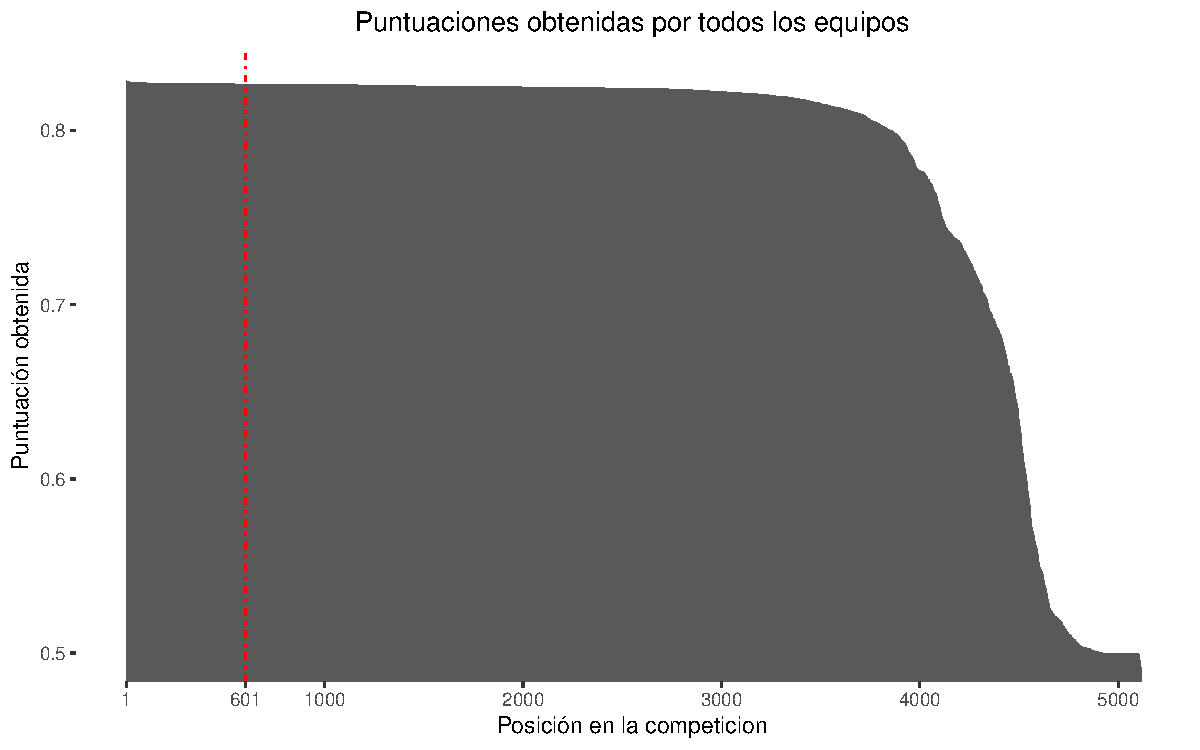
\includegraphics[width=\textwidth]{Z_07_01_Posicion_competicion.pdf}
    \caption{Posición final en la competición.}
    \end{center}
\end{figure}

\newpage

\section{Conclusiones}
Al comenzar este trabajo se plantearon una serie de objetivos. Los resultados finales son en general satisfactorios. Los problemas más importantes que han ido surgiendo se han solucionado y el modelo final es de un nivel similar a la solución ganadora. Para el futuro pienso que todavía queda margen para la mejora: algunos de los algoritmos que he venido utilizando pueden optimizarse, algunos procesos pueden automatizarse y hay algunas técnicas como las redes neuronales que no he implementado y que podrían aportar mejoras. Falta todavía un punto de excencia para llegar a obtener los mejores resultados. 

A nivel personal he aprendido muchísimo. Quiero destacar el nivel que he llegado a conseguir programando en el lenguaje R. Este problema era mucho más complejo que aquellos que había visto hasta ahora. Ha sido todo un reto personal. Veo también una evolución muy positiva cuando comparo los resultados que obtenía al principio del proyecto con los que he llegado a conseguir. 

Por último quiero volver a agradecer a mi tutor, profesores, familiares y amigos el apoyo y los consejos que me han dado. 







\newpage


\appendix

\section{Anexo. Código regresión logística}
{\scriptsize
\begin{verbatim}
library(ROSE)

set.seed(1117)

'%ni%' <- Negate('%in%') 

train <- read.csv("train.csv", sep=",", header = TRUE, dec=".")
test <- read.csv("test.csv", sep=",", header = TRUE, dec=".")

vars <- c("var15_s", "saldo_var30", "num_med_var22_ult3_s", "imp_op_var39_efect_ult3_s", "num_var24",
          "saldo_medio_var5_hace2", "num_ent_var16_ult1_s", "ind_var30_0_s", "num_aport_var13_hace3",
          "saldo_var37", "num_var22_ult3", "saldo_medio_var17_hace2_s", "ind_var13_largo_s", "num_var40_s", 
          "saldo_medio_var44_hace2", "num_sal_var16_ult1", "num_op_var39_efect_ult3", "num_var22_ult1_s", 
          "imp_op_var41_efect_ult1_s", "imp_op_var40_efect_ult1_s", "imp_ent_var16_ult1", "ind_var24")

train$val_cero <- rowSums(train == 0)
test$val_cero <- rowSums(test == 0)

log_vars <- c("saldo_medio_var12_hace2","saldo_medio_var12_hace3","saldo_medio_var12_ult1",
              "saldo_medio_var12_ult3","saldo_medio_var13_corto_hace2","saldo_medio_var13_corto_hace3",
              "saldo_medio_var13_corto_ult1","saldo_medio_var13_corto_ult3","saldo_medio_var17_ult3",
              "saldo_medio_var13_largo_hace2","saldo_medio_var13_largo_hace3","saldo_var25",
              "saldo_medio_var13_largo_ult1","saldo_medio_var13_largo_ult3","saldo_medio_var29_ult3",
              "saldo_medio_var13_medio_hace2","saldo_medio_var13_medio_hace3", "saldo_medio_var5_ult3",
              "saldo_medio_var13_medio_ult1","saldo_medio_var13_medio_ult3","saldo_medio_var33_ult3",
              "saldo_medio_var17_hace2","saldo_medio_var17_hace3","saldo_medio_var17_ult1",
              "saldo_medio_var29_hace2","saldo_medio_var29_hace3","saldo_medio_var29_ult1","saldo_var46",
              "saldo_medio_var33_hace2","saldo_medio_var33_hace3","saldo_medio_var33_ult1","saldo_var5",
              "saldo_medio_var44_hace2","saldo_medio_var44_hace3","saldo_medio_var44_ult1","saldo_var6",
              "saldo_medio_var44_ult3","saldo_medio_var5_hace2","saldo_medio_var5_hace3","saldo_var24",
              "saldo_medio_var5_ult1","saldo_medio_var8_hace2","saldo_medio_var8_hace3","saldo_var32",
              "saldo_medio_var8_ult1","saldo_medio_var8_ult3","saldo_var1","saldo_var12", "saldo_var8",
              "saldo_var13","saldo_var13_corto","saldo_var13_largo","saldo_var13_medio", "var38",
              "saldo_var14","saldo_var17","saldo_var18","saldo_var2_ult1","saldo_var20","saldo_var44",
              "saldo_var26","saldo_var27","saldo_var28","saldo_var29","saldo_var30","saldo_var31",  
              "saldo_var33","saldo_var34","saldo_var37","saldo_var40","saldo_var41","saldo_var42") 

for (i in log_vars){
  train[ , i] <- log(train[ , i])
}

for (i in log_vars){
  test[ , i] <- log(test[ , i])
}

for (var in names(train)){
  if (length(unique(train[[var]])) == 1) {
    train[[var]] <- NULL
    test[[var]] <- NULL
  }
}

var_par <- combn(names(train), 2, simplify = F)
to_delete <- c()
for(par in var_par) {
  v1 <- par[1]
  v2 <- par[2]
  
  
  if (!(v1 %in% to_delete) & !(v2 %in% to_delete)){
    if (all(train[[v1]] == train[[v2]])){
      to_delete <- c(to_delete, v2)
    }
  }
}

set_vars <- setdiff(names(train), to_delete)
train <- train[,-which(names(train) %in% to_delete)]
test <- test[,-which(names(test) %in% to_delete)]

train[train$var3 == -999999, "var3"] <- 37
train[train$var36 == 99, "var36"] <- 4
train[train$delta_imp_aport_var13_1y3 == 9999999999, "delta_imp_aport_var13_1y3"] <- 6
train[train$delta_imp_aport_var17_1y3 == 9999999999, "delta_imp_aport_var17_1y3"] <- 2
train[train$delta_imp_compra_var44_1y3 == 9999999999, "delta_imp_compra_var44_1y3"] <- 7
train[train$delta_imp_reemb_var13_1y3 == 9999999999, "delta_imp_reemb_var13_1y3"] <- 1
train[train$delta_imp_reemb_var17_1y3 == 9999999999, "delta_imp_reemb_var17_1y3"] <- 1
train[train$delta_num_aport_var13_1y3 == 9999999999, "delta_num_aport_var13_1y3"] <- 2
train[train$delta_num_aport_var17_1y3 == 9999999999, "delta_num_aport_var17_1y3"] <- 3
train[train$delta_num_compra_var44_1y3 == 9999999999, "delta_num_compra_var44_1y3"] <- 4
train[train$delta_num_compra_var44_1y3 == 4, "delta_num_compra_var44_1y3"] <- 3
train[train$delta_num_reemb_var13_1y3 == 9999999999, "delta_num_reemb_var13_1y3"] <- 1
train[train$delta_num_reemb_var17_1y3 == 9999999999, "delta_num_reemb_var17_1y3"] <- 1
train <- do.call(data.frame,lapply(train, function(x) replace(x, is.infinite(x), NA)))
train[is.na(train)] <- 0

train <- ROSE(TARGET ~ ., data=train)$data
TARGET <- train$TARGET
train.s <- data.frame(scale(train))
colnames(train.s) <- paste0(colnames(train.s),"_s")
train <- dplyr::bind_cols(train, train.s)

testID <- test$ID

test[test$var3 == -999999, "var3"] <- 37
test[test$var36 == 99, "var36"] <- 4
test[test$delta_imp_aport_var13_1y3 == 9999999999, "delta_imp_aport_var13_1y3"] <- 6
test[test$delta_imp_aport_var17_1y3 == 9999999999, "delta_imp_aport_var17_1y3"] <- 2
test[test$delta_imp_compra_var44_1y3 == 9999999999, "delta_imp_compra_var44_1y3"] <- 7
test[test$delta_imp_reemb_var13_1y3 == 9999999999, "delta_imp_reemb_var13_1y3"] <- 1
test[test$delta_imp_reemb_var17_1y3 == 9999999999, "delta_imp_reemb_var17_1y3"] <- 1
test[test$delta_num_aport_var13_1y3 == 9999999999, "delta_num_aport_var13_1y3"] <- 2
test[test$delta_num_aport_var17_1y3 == 9999999999, "delta_num_aport_var17_1y3"] <- 3
test[test$delta_num_compra_var44_1y3 == 9999999999, "delta_num_compra_var44_1y3"] <- 4
test[test$delta_num_reemb_var13_1y3 == 9999999999, "delta_num_reemb_var13_1y3"] <- 1
test[test$delta_num_reemb_var17_1y3 == 9999999999, "delta_num_reemb_var17_1y3"] <- 1
test <- do.call(data.frame,lapply(test, function(x) replace(x, is.infinite(x), NA)))
test[is.na(test)] <- 0
test.s <- data.frame(scale(test))

colnames(test.s) <- paste0(colnames(test.s),"_s")
test <- dplyr::bind_cols(test, test.s)

train <- train[,which(names(train) %in% vars)]
test <- test[,which(names(test) %in% vars)]

train$TARGET <- TARGET
logitmod <- glm(as.formula(paste("TARGET ~ ", paste(vars, collapse=" + "))), 
                family = binomial, data = train)
predictions <- predict(logitmod, newdata=test, type="response") 
y_pred_num <- ifelse(predictions > 0.5, 1, 0)
table(y_pred_num)

write.csv(data.frame(ID=testID, TARGET=predictions), 
          file = "Logit_ROSE_binded_22vars.csv",
          row.names=FALSE)
\end{verbatim}
}

\newpage

\section{Anexo. Código KNN}
{\scriptsize
\begin{verbatim}
library(caret)

'%ni%' <- Negate('%in%') 

train <- read.csv("train.csv", sep=",", header = TRUE, dec=".")
test <- read.csv("test.csv", sep=",", header = TRUE, dec=".")

set.seed(1117)

vars <- c("imp_trans_var37_ult1", "num_var42", "saldo_var13", "saldo_var25", "ind_var30_0", 
          "saldo_medio_var13_corto_ult3", "imp_op_var40_efect_ult1", "saldo_var13_corto", 
          "var3", "ind_var13_largo")

train <- upSample(x=train[,colnames(train) %ni% "TARGET"], y=as.factor(train$TARGET), yname="TARGET")
TARGET <- train$TARGET
train <- train[,which(names(train) %in% vars)]
train <- data.frame(scale(train))

testID <- test$ID
test <- test[,which(names(test) %in% vars)]
test <- data.frame(scale(test))

fit <- knn3(as.matrix(train), as.factor(TARGET), k=5, prob = TRUE)  
predictions <- predict(fit, as.matrix(test), type="class")
table(predictions)

write.csv(data.frame(ID=testID, TARGET=predictions), 
          file = "KNN_upsampling_10vars_5k.csv",
          row.names=FALSE)
\end{verbatim}
}

\newpage

\section{Anexo. Código clasificador bayesiano ingenuo}
{\scriptsize
\begin{verbatim}
library(caret)
library(DMwR)
library(naivebayes)

set.seed(1117)

'%ni%' <- Negate('%in%') 

train <- read.csv("train.csv", sep=",", header = TRUE, dec=".")
test <- read.csv("test.csv", sep=",", header = TRUE, dec=".")
train <- train
testID <- test$ID
TARGET <- train$TARGET

vars <- c("ind_var30", "num_var37_med_ult2", "num_op_var40_efect_ult1", "var15", 
          "imp_op_var40_ult1", "ind_var5_0", "num_var45_hace3", "var38")

rows_train <- createDataPartition(train$TARGET, p=1, list=FALSE)
train <- train[rows_train, ]
train$TARGET <- as.factor(TARGET)
train <- SMOTE(TARGET ~ train, train, perc.over = 100, perc.under=200)
TARGET <- train$TARGET
train <- train[,-which(names(train) %in% c("ID", "TARGET"))]

train <- data.frame(scale(train))
test <- data.frame(scale(test))

train <- train[,which(names(train) %in% vars)]
test <- test[,which(names(test) %in% vars)]

nb_mod <- naive_bayes(x=train, y=TARGET)

pred_final <- predict(nb_mod, newdata=test)
pred_final <- as.numeric(pred_final)
pred_final[pred_final==1] <- 0
pred_final[pred_final==2] <- 1

write.csv(data.frame(ID=testID, TARGET=pred_final), 
          file = "Bayes_SMOTE_7vars.csv",
          row.names=FALSE)

\end{verbatim}
}

\newpage

\section{Anexo. Código máquina de soporte vectorial}
{\scriptsize
\begin{verbatim}
library(caret)
library(DMwR)

set.seed(1117)

'%ni%' <- Negate('%in%') 

train <- read.csv("train.csv", sep=",", header = TRUE, dec=".")
test <- read.csv("test.csv", sep=",", header = TRUE, dec=".")
train <- train
testID <- test$ID
TARGET <- train$TARGET

vars <- c("num_var4", "saldo_var40", "ind_var41_0", "ind_var37_cte", 
  "ind_var1_0", "imp_op_var40_ult1", "imp_sal_var16_ult1", 
  "ind_var17", "num_var24", "ind_var1", "ind_var40", "ind_var24")

train <- downSample(x=train[,colnames(train) %ni% "TARGET"], 
                    y=as.factor(train$TARGET), yname="TARGET")
TARGET <- train$TARGET
train <- train[,-which(names(train) %in% c("ID", "TARGET"))]
train <- data.frame(scale(train))
test <- data.frame(scale(test))


train <- train[,which(names(train) %in% vars)]
test <- test[,which(names(test) %in% vars)]

ctrl <- trainControl(method = "none", search="grid", allowParallel = TRUE, 
                     summaryFunction=twoClassSummary, classProbs=TRUE)
grid <- expand.grid(C=c(1), scale=c(0.1), degree=c(3))
train$TARGET <- make.names(TARGET)
mod <- train(TARGET ~ ., data=train, method="svmPoly", metric="ROC", 
             tuneGrid = grid, trControl=ctrl)

predictions <- predict(mod, test)
predictions <- as.numeric(predictions)
predictions[predictions==1] <- 0
predictions[predictions==2] <- 1
table(predictions)

write.csv(data.frame(ID=testID, TARGET=predictions), 
          file = "SVM_downsampling_12vars_C1_sc0.1_d3.csv",
          row.names=FALSE)
\end{verbatim}
}
\newpage

\section{Anexo. Código Random Forest}
{\scriptsize
\begin{verbatim}
library(caret)

set.seed(1117)

'%ni%' <- Negate('%in%') 

#registerDoMC(cores=8)

train <- read.csv("train.csv", sep=",", header = TRUE, dec=".")
test <- read.csv("test.csv", sep=",", header = TRUE, dec=".")

TARGET <- train$TARGET
testID <- test$ID

train$val_cero <- rowSums(train == 0)
test$val_cero <- rowSums(test == 0)

vars<- c("var15", "saldo_var30", "num_var22_ult3", "num_meses_var5_ult3", "val_cero", 
         "ind_var30_0", "num_aport_var13_hace3", "var38", "num_var22_ult1", "saldo_var5",
         "num_var35", "ind_var41_0", "saldo_medio_var5_ult3", "ind_var43_recib_ult1", 
         "ind_var43_emit_ult1", "num_var5", "ind_var37_cte", "num_var41_0", "num_var14",
         "saldo_medio_var12_hace2", "ind_var37_0", "ind_var8_0", "ind_var30", 
         "num_op_var39_comer_ult1", "num_var4", "imp_aport_var17_ult1", "ind_var19",
         "num_meses_var8_ult3", "imp_ent_var16_ult1", "num_op_var41_comer_ult1", 
         "imp_op_var41_ult1", "num_meses_var44_ult3", "ind_var14",  "ind_var9_ult1", 
         "saldo_medio_var8_ult3", "saldo_medio_var8_hace2", "imp_op_var41_comer_ult3", 
         "delta_imp_aport_var17_1y3")  

train <- train[,which(names(train) %in% vars)]
test <- test[,which(names(test) %in% vars)]


ctrl <- trainControl(method="none", classProbs=TRUE,
                     summaryFunction=multiClassSummary)

grid <- expand.grid(mtry = c(12), splitrule="gini")

train$TARGET <- make.names(TARGET)

parRF_mod <- train(as.formula(paste(paste("TARGET ~", paste(vars, collapse=" + ")),sep = "")), 
				   data=train, method= "ranger", metric="ROC", tuneGrid=grid, trControl=ctrl)

predictions <- predict(parRF_mod, test)

predictions <- as.numeric(predictions)
predictions[predictions==1] <- 0
predictions[predictions==2] <- 1

table(predictions)

write.csv(data.frame(ID=testID, TARGET=predictions), 
          file = "RF_descompensado_39vars_mtry12.csv",
          row.names=FALSE)
\end{verbatim}
}

\newpage

\section{Anexo. Código XGBoost}
{\scriptsize
\begin{verbatim}
library(xgboost)
library(Matrix)

set.seed(1117)

train <- read.csv("train.csv", sep=",", header = TRUE, dec=".")
test <- read.csv("test.csv", sep=",", header = TRUE, dec=".")


TARGET <- train$TARGET
testID <- test$ID
train <- train[,-which(names(train) %in% c("ID", "TARGET"))]
test <- test[,-which(names(test) %in% c("ID"))]

train$val_cero <- as.integer(rowSums(train == 0))
test$val_cero <- as.integer(rowSums(test == 0))

for (var in names(train)){
  if (length(unique(train[[var]])) == 1) {
    train[[var]] <- NULL
    test[[var]] <- NULL
  }
}

var_par <- combn(names(train), 2, simplify = F)
to_delete <- c()
for(par in var_par) {
  v1 <- par[1]
  v2 <- par[2]
  
  if (!(v1 %in% to_delete) & !(v2 %in% to_delete)){
    if (all(train[[v1]] == train[[v2]])){
      to_delete <- c(to_delete, v2)
    }
  }
}

set_vars <- setdiff(names(train), to_delete)
train <- train[,-which(names(train) %in% to_delete)]
test <- test[,-which(names(test) %in% to_delete)]

train$TARGET <- TARGET

train <- sparse.model.matrix(TARGET ~ ., data = train)
train <- xgb.DMatrix(data = train, label = TARGET)

parametros <- list(objective="binary:logistic", booster="gbtree", 
                   eval_metric="auc", eta=0.008235294, subsample=0.75, 
                   colsample_bytree=0.7, min_child_weight=0.6, max_depth=7)

modelo <- xgb.train(params=parametros, data=train, nrounds=850, maximize=FALSE)

test$TARGET <- -1
test <- sparse.model.matrix(TARGET ~ ., data = test)

predictions <- predict(modelo, test)

write.csv(data.frame(ID=testID, TARGET=predictions), 
          file = "XGB_tree_1826.csv",
          row.names=FALSE)
\end{verbatim}
}

\newpage

\section{Anexo. Cuadro resumen}

\begin{table}[!htbp]
\center
\renewcommand{\arraystretch}{1.3}
\begin{adjustbox}{angle=90}
	\resizebox{8.8in}{!}{\begin{tabular}{rcccccc}
	  \hline
	  \hline
	 & Regresión logística & KNN & Naïve Bayes & SVM & Random Forest & XGBoost \\ 
	  \hline
	  \hline
		TRANSFORMACIONES &  &  &  &  &  &  \\ 
		\hline 
		Estandarizado & X & X & X & X &  &  \\ 
		Logaritmo & X &  &  &  &  &  \\ 
		Eliminación constantes & X &  &  &  &  &  \\ 
		Datos perdidos & X &  &  &  &  & X  \\ 
		Centrado/Normalizado & X &  &  &  &  &  \\ 
		\hline
		DESCOMPENSACIÓN &  &  &  &  &  &  \\ 
		\hline
		Downsampling &  &  &  & X &  &  \\ 
		Upsampling &  & X &  &  &  &  \\ 
		Smote &  &  & X &  &  &  \\ 
		ROSE & X &  &  &  &  &  \\ 
		\hline
		SELECCIÓN VARIABLES &  &  &  &  &  &  \\
		\hline 
		Selección sucesiva & X & X & X & X &  &  \\ 
		Variables importantes &   &   &   &   & X &  \\
		Todas las variables &  &  &  &  &   & X  \\
		\hline 
		VALIDACIÓN &  &  &  &  &  &  \\
		\hline 
		K-fold CV &  &  &  & X & X & X  \\ 
		Random CV & X & X & X &  &  &  \\ 
	    \hline
	    \hline
		PUNTUACIÓN OBTENIDA &  &  &  &  &  &  \\ 
		\hline
	    \hline
		Pública & 0.797883 & 0.504230 & 0.660662 & 0.677769 & 0.619606 & 0.840522 \\ 
		Privada & 0.781125 & 0.500277 & 0.688245 & 0.653400 & 0.598594 & 0.826565 \\ 
	   \hline
	   \hline
	\end{tabular}}
	
\end{adjustbox}
\caption{Mejores resultados AUC obtenidos con cada algoritmo en kaggle.com}
\end{table}


\newpage

\begingroup
    \setlength{\bibsep}{10pt}
    \setstretch{1}
    \bibliography{bibliog}
\endgroup



%FIN DEL DOCUMENTO
\end{document}